
\documentclass[conference]{IEEEtran}
\IEEEoverridecommandlockouts
% The preceding line is only needed to identify funding in the first footnote. If that is unneeded, please comment it out.
\usepackage{cite}
%\usepackage{caption}
%\usepackage{subcaption}
\usepackage{tikz}
\usetikzlibrary{shapes.geometric,arrows, positioning, fit, calc}
\usepackage{amsmath,amssymb,amsfonts}
%\usepackage{algorithmic}
%\usepackage{algorithm}
\usepackage{graphicx}
%\usepackage{xcolor}
%\usepackage{epsfig}
%\usepackage{mathptmx}
%\usepackage{textcomp}
%\usepackage{mathtools}
%\usepackage{lipsum}
%\usepackage{gensymb}
\usepackage{float}
\usepackage{epstopdf}

\tikzstyle{computing} = [draw, rectangle, fill=white!50, rounded corners, node distance=3em, minimum height=3em]

\tikzstyle{io} = [rectangle, draw, trapezium right angle=110, rounded corners,
                  fill=red!20, node distance=5em, minimum height=2.9em]

\tikzstyle{calculate} = [diamond, draw, trapezium right angle=110, rounded corners,
                  fill=green!20, node distance=1.9cm, minimum height=2.9em]

\tikzstyle{hardware} = [rectangle, draw, trapezium right angle=110, rounded corners,
                  fill=blue!20, node distance=1.9cm, minimum height=2.9em]

\tikzstyle{external} = [rectangle, draw, trapezium right angle=110, rounded corners,
                  fill=gray!20, node distance=1.9cm, minimum height=2.9em]
\tikzstyle{line} = [draw, -latex']

\tikzstyle{function} = [rectangle, draw, fill=green!20, node distance=1.9cm, minimum height=2.9em]


\def\BibTeX{{\rm B\kern-.05em{\sc i\kern-.025em b}\kern-.08em	
    T\kern-.1667em\lower.7ex\hbox{E}\kern-.125emX}}	

    \title{Project Report*\\	
    {\footnotesize \textsuperscript{*}As a fulfilment to the course: "Project course name",	
     D7039E \& E7032E. Lecturer: Jan van Deventer.}	
    %%\thanks{Identify applicable funding agency here. If none, delete this.}	
    }	

    \author{\IEEEauthorblockN{Martin Blaszczyk, Edward Cedegård, Niklas Dahlquist, Edward Källstedt, Albin Martinsson, Måns Norell}	
    \IEEEauthorblockA{\textit{Computer Science, Electrical and Space Engineering Dept.} \\	
    \textit{Lule{\aa} University of Technology}\\	
    Lule\aa, Sweden \\	
    \{marbla-6, edwced-4, nikdah-6, edwkll-7, mnsnor-5, albmar-6\}@student.ltu.se}	
    }	
\date{\today}	

\begin{document}	
\maketitle	
\begin{abstract}	
\end{abstract}	

\section{Introduction}	
\section*{Background and motivation}
Self explanatory. 
\section*{Contributions}
How does this report contribute. Are there any novel solutions?
\section*{Structure}
The overall structure of the report
	

\section{Arrowhead}	
\section*{Arrowhead}
What is it?
\section*{Extras}
More in depth about the strucutre of the Arrowhead implementation. Flow diagrams etc. 	


\section{Communication}
\section*{Communication}
Unlike most servo motors Dynamixel uses digital packet communication instead of pulse-width modulation (PWM) signals.
By grouping data into different packages and transmitting it as a bundle.
This in turn opens up for many possibilities since the motors responds to commands,
have built in control functions together with memory allocation on the motor itself.
Dynamixel recommends two different setups for communication,
either by using a Tri-state-buffer to construct your own communication bridge  based on Universal asynchronous receiver-transmitter setup (UART). Or by using their own solution called U2D2.
In essense, the U2D2 uses the same protocol but also enables for USB communication between the controller and Dynamixels \cite{robotis}. 

\subsection{UART full duplex to half duplex}
UART communication scheme works by connecting the transmitter pin (Tx) of the Jetson Nvidia Nano microcontroller (MCU)
directly to the receiver pin (Rx) of the motors and vice versa.
UART communication can be setup into three different ways of communication.
Full duplex, half duplex and simplex.
Full duplex allows for data communication both ways simultaneously.
Half duplex only allows for one way communication at any given time, by either sending or receiving.
Simplex communication is static, meaning communication is always one direction.
\newline
Full duplex and half duplex are not directly compatible. 
If the MCU and Dynamixel motors are connected directly,
since the MCU sends and receive data simultaneously it will occupy the transmission line indefinitely and the Dynamixel won't be able to tell when the messages stop. 
This phenomena is known as chatter. 
The solution for this is to implement a tri-state-buffer circuit converting the full system to half duplex.

\subsection{Tri-state-buffer}

A tri-state-buffer dictates when the MCU is allowed to communicate with the motors. This explained  by figure \ref{duplex}.
By controlling the direction pin (GPIO pin),
we can direct the flow of data. 
If the direction pin is pulled high we simultaneously allow for transmission from the MCU (Tx) to the motors and disable the MCU receiver pin (Rx).
A crucial part is timing, the direction pin must be pulled high long enough for the data to transfer through the buffer otherwise information is lost.
A logic analyzer will give this information and is recommended to use in conjugation with the tri-state-buffer for tuning.

\subsection{Data package - structure of message}
The protocol allows for a size of 8 bits per message between the MCU and motors. 
The two types message structures is represented by the figures below \ref{instr} and \ref{return}.
For more information how to interpret the structure use dynamixels own documentation ().

\subsubsection{Instruction package}
Instruction package carries commands from the controller to the motor.
An abundance of support is included,
from changing statics parameters like torque, baud-rate or id of each individual unit or different actions,
for example move to this location with this speed.
The structure of the message is represented in figure \ref{instr} and table \ref{instr_table} describes the structure from left to right. 

\begin{table}[H]
    \centering
    \caption{Explanation of parameters in instruction packadge}
    \begin{tabular}{c | c c c c c}
        \(OXFF\) & Indicates start of incoming packet  \\
        \hline
        \(ID\) & Specific ID of each unit  \\
        \hline
        \(Length\) & Length of message \\
        \hline
        \(Param\) & Used for additional information  \\
        \hline
        \(Check sum\) & Calculate length of packet \\
        \hline
    \end{tabular}
    \label{instr_table}
\end{table}

\begin{figure}[H]
    \centering
    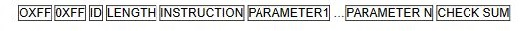
\includegraphics[width=\columnwidth]{chapters/img/instruction_packadge.JPG}
    \label{instr}
    \caption{Structure of instruction message.}
\end{figure}
%img/instruction_packadge

\subsubsection{Status package}
Status packet contains the response from the Dynamixel to the controller after receiving a instruction.
The structure is almost the same as the instruction package.
However, one difference is the the message confirms the status of sent instructions including an error if one occurs.
The structure is represented in figure \ref{return} and Dynamixels support page \cite{protocol1} gives more information how to read the error messages.

\begin{figure}[H]
    \centering    
    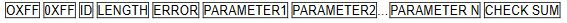
\includegraphics[width=0.7\columnwidth]{chapters/img/return_packadge.JPG}
    \label{return}
    \caption{Structure of return message.}
\end{figure}

\subsection{Motor communication}
Dynamixel provides a lot of support for lower level programming using instructions and reading return messages with documentation support, as stated above
. However, there is also support for higher level and more user friendly programming languages like Python,
C and third-party libraries by using Dynamixels own software development kit called DYNAMIXEL SDK \cite{dynamixel_SDK}.




\section{Modeling}


%%%%%%%%%%%%%%%% arm kinematics %%%%%%%%%%%%%%

\begin{figure}[H]
    \centering
    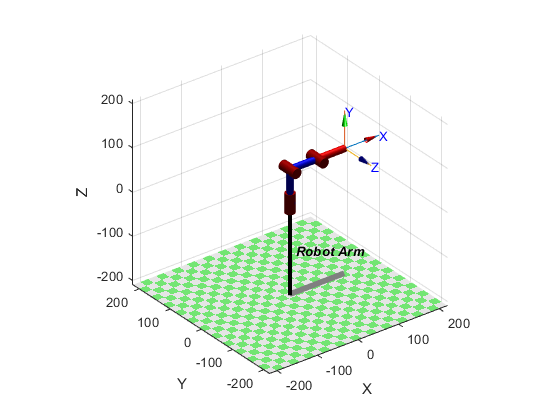
\includegraphics[width=0.7\columnwidth]{chapters/img/robot_arm.png}
    \caption{Placeholder image for the robotic arm?.}
    \label{fig:robotic_manipulator_general}
\end{figure}


\section*{Manipulator Kinematics} %Niklas
Kinematics is what describes the motion of rigid bodies and points in space. 

\subsection*{Backgroud}
\subsection*{Rigid body transformation}
In general any position can be described by translation along three axes and rotation along these same axes. These translations/rotations can be described by a matrix
\begin{equation}
    T = 
    \begin{bmatrix}
        R & d \\
        \bf{0} & 1
    \end{bmatrix}
\end{equation}
where \(R\) is a 3 x 3 rotation matrix and \(d\) a 3 x 1 translation matrix. This implies that any transformation could be characterized by six parameters, three for the translation and three for the rotation. \cite{spong}


\subsection*{Denavit-Hartenberg Convention}
A common approach for selecting the coordinate frames of reference for each joint in a robotic arm is the Denavit-Hartenberg convention. This allows the transformation matrix for each joint to be expressed as
\begin{equation}
    A_i = Rot_{z}(\theta_i) \cdot Trans_{z}(d_i) \cdot Trans_{x}(a_i) \cdot Rot_{z}(\alpha_i)
    \label{eqn:DH-transformation}
\end{equation}
that consists of the four basic transformations
\begin{equation}
    Rot_z(\theta_i) = 
    \begin{bmatrix}
        cos(\theta_i) & -sin(\theta_i) & 0 & 0 \\
        sin(\theta_i) & cos(\theta_i) & 0 & 0 \\
        0 & 0 & 1 & 0 \\
        0 & 0 & 0 & 1
    \end{bmatrix}
\end{equation}
\begin{equation}
    Trans_z(d_i) = 
    \begin{bmatrix}
        1 & 0 & 0 & 0 \\
        0 & 1 & 0 & 0 \\
        0 & 0 & 1 & d_i \\
        0 & 0 & 0 & 1
    \end{bmatrix}
\end{equation}
\begin{equation}
    Trans_x(\alpha_i) = 
    \begin{bmatrix}
        1 & 0 & 0 & \alpha_i \\
        0 & 1 & 0 & 0 \\
        0 & 0 & 1 & 0 \\
        0 & 0 & 0 & 1
    \end{bmatrix}
\end{equation}
\begin{equation}
    Rot_z(\theta_i) = 
    \begin{bmatrix}
        1 & 0 & 0 & 0 \\
        0 & cos(\alpha_i) & -sin(\alpha_i) & 0 \\
        0 & sin(\alpha_i) & cos(\alpha_i) & 0 \\
        0 & 0 & 0 & 1
    \end{bmatrix}.
\end{equation}


Where the parameters \(\theta_i\), \(a_i\), \(d_i\) and \(\alpha_i\), known as DH-parameters, characterize each joint. To allow the transformation for each joint to be represented by only four parameters, compared to the six parameters that is required in general, there are some restrictions on how the coordinate frames can be chosen. To comply with the DH-convention, the following must be satisfied.
\begin{itemize}
    \item The axis \(x_{1}\) is perpendicular to the axis \(z_0\)
    \item The axis \(x_{1}\) intersects the axis \(z_0\)
\end{itemize}
where it is assumed that two frames are given, frame 0 and frame 1, and the transformation from equation \ref{eqn:DH-transformation} transforms a coordinate from frame 1 into a coordinate in frame 0.\cite{spong}



\subsection*{Kinematic Chain} %A1*A2*...
A robotic manipulator can be described by a set of joints with links between them where a homogeneous transformation matrix \(A_i\) that describes the transformation with respect to the previous joint exists for each joint. This means that a transformation that describes the position and orientation of joint \(j\) with respect to a joint \(i\) to a can be found by a transformation matrix \cite{spong}
\begin{equation}
    \begin{cases}
        T_j^i = A_{i+1}A_{i+2}...A_{j-1}A_{j}, \text{  if \(i < j\) } \\
        T_j^i = I, \text{  if \(i = j\) } \\
        T_j^i = (T_i^j)^{-1}, \text{  if \(i > j\) }
    \end{cases}
    \label{eqn:Kinematic_chain_spong}
\end{equation}



\subsection*{Forward Kinematics}
Forward kinematics is the problem of finding the position and orientation of the end effector.

Since a manipulator can be seen as a kinematic chain the problem of finding the position and orientation of the end effector can be solved by finding the transformation matrices in equation \ref{eqn:Kinematic_chain_spong}.



\subsection*{Inverse Kinematics}
The problem of finding the joint states required for achieving a desired pose is called inverse kinematics. For some simple kinematic chains an analytical solution exists, but in general a numerical approach might be required. 

%we have for joints, three needed for position. geometric approach for finding the position. then joint for is used to control the pitch of the EOF





\subsection*{Workspace}
A robotic manipulator will not be able to reach all points in space since it has a fixed size. It will not even be able to reach all mathematically reachable points since each joint (usually) have some restrictions on how it can rotate/translate. The physically reachable space is defined as the workspace of the manipulator. %source might be needed here
\\




%%%%%%%%%%%%%%%%%%%%%%%%%%%%%%%%%%%%%%%%%%%%%%%%%%%%%%%%%%%%%%%%
%%%%%%%%%%%%%% Kinematics Implementation %%%%%%%%%%%%%%%%%%%%%%%
%%%%%%%%%%%%%%%%%%%%%%%%%%%%%%%%%%%%%%%%%%%%%%%%%%%%%%%%%%%%%%%%
\subsection*{Implementation}

\subsection*{Denavit-Hartenberg Convention}
In table \ref{tab:DH-table} the DH-parameters that was used for the robotic manipulator, seen in figure \ref{fig:robotic_manipulator_general}, are listed.
\begin{table}[H]
    \centering
    \caption{The Denavit-Hartenberg parameters used for the robotic manipulator.}
    \begin{tabular}{c | c c c c c}
        \(i\) & \(\theta_i\) [rad] & \(d_i\) [mm] & \(a_i\) [mm] & \(\alpha_i\) [rad] \\
        \hline
        \(1\) & \(\theta_1\) & \(75\) & \(0\) & \(\pi / 2\) \\
        \(2\) & \(\theta_2\) & \(0\) & \(67.5\) & \(0\) \\
        \(3\) & \(\theta_3\) & \(0\) & \(67.5\) & \(0\) \\
        \(4\) & \(\theta_4\) & \(0\) & \(65\) & \(0\) \\
    \end{tabular}
    \label{tab:DH-table}
\end{table}



\subsection*{Forward Kinematics}
The transformation matrices from equation \ref{eqn:DH-transformation} for each joint can be multiplied together
\begin{equation}
    T_{end} = A_1 \cdot A_2 \cdot A_3 \cdot A_4
\end{equation}
where \(A_1\) - \(A_4\) are calculated from equation \ref{eqn:DH-transformation} to find the pose \(T_{end}\) of the end effector and thereby solving the forward kinematic problem.


\subsection*{Inverse Kinematics}
To solve the inverse kinematics for the position of a three joint manipulator a geometric method can be used to find an analytical solution. The required angles to achieve a desired position \((x_d, y_d, z_d)\) in an elbow-up configuration are \cite{Lec14_mit_Manipulation}

\begin{equation}
    \begin{cases}
        \theta_1 = Atan(x, y) \\
        \theta_3 = Atan(D, +\sqrt{1 - D^2}) \\
        \theta_2 = Atan(\sqrt{x_d^2 + y_d^2}, z_d - d_1) \\- Atan(a_2 + a_3 \cdot D, a_3 \cdot \sqrt{1 - D^2}) %fix
    \end{cases}
\end{equation}
where \(Atan(x, y)\) is the two argument arctangent function \cite{inverse_tangent_wolfram} and 

\begin{equation}
    D = \frac{x_d^2 + y_d^2 + (z_d - d_1)^2 - a_2^2 - a_3^2}{2 a_2 a_3}
\end{equation}
and \(a_2\), \(a_3\), and \(d_1\)   are the corresponding DH-parameters.



\subsection*{Workspace}
The robotic manipulator seen in figure \ref{fig:robotic_manipulator_general} has the following limitations for the first three joints
\begin{equation}
    \begin{cases}
        -100^\circ < \theta_1 < 100^\circ \\
        -100^\circ < \theta_2 < 100^\circ \\
        -100^\circ < \theta_3 < 100^\circ 
    \end{cases}
    \label{eqn:workspace_limits_angles}
\end{equation}
and a simulated 2D slice of the workspace can be seen in figure \ref{fig:workspace_simulated}. The full workspace can be formed by rotating this 2D slice around the z-axis according to the limitations on \(\theta_1\) from equation \ref{eqn:workspace_limits_angles}.


\begin{figure}[H]
    \centering
    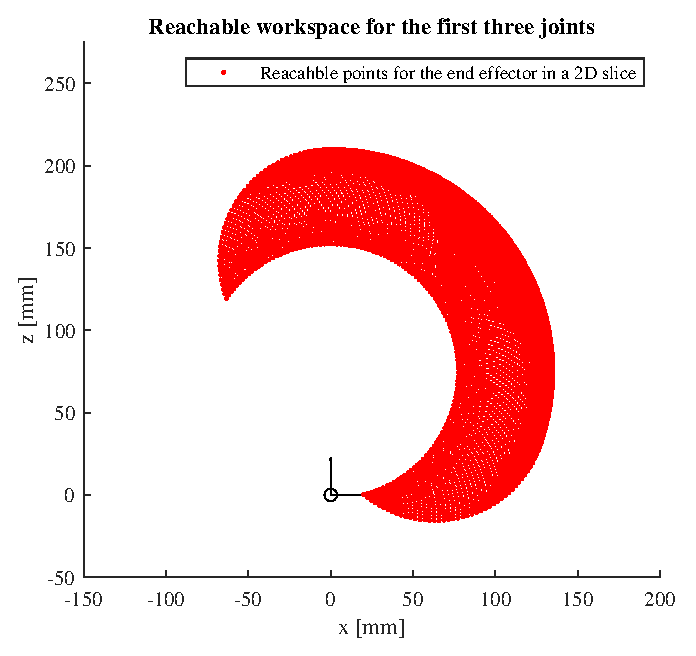
\includegraphics[width=0.7\columnwidth]{chapters/img/workspace.eps}
    \caption{A simulated 2D slice of the workspace for the three jointed manipulator.}
    \label{fig:workspace_simulated}
\end{figure}
%chapters/img/workspace.eps




%%%%%%%%%%%%%%%% arm kinematics end %%%%%%%%%%%%%%













\section*{Base}

The motors will be connected to tracks on the robot and can therefore be modelled as two wheels connected with a rod, as seen in figure \ref{fig:base_math_model}.\\ 
Deriving a mathematical model is straight forward if we can read the encoders from the motors. From the encoders we would be able to get both the length the robot has traveled and more importantly the individual speed each motor rotates with. The speed for the individual motor is given by: 

\begin{equation}
    v_m=\frac{2\pi r_{wh}/N_{enc}}{\Delta t}
    \label{eq:base_system_eq1}
\end{equation}

\noindent Where $N_{enc}$ is the number of encoders on the motor, $r_{wh}$ is the radius of the driving wheel and thickness of the track and $\Delta t$ is the time between the previous encoder reading and the most recent one. By doing this for both the left and right motor we can find how fast the robot is moving along the line by:

\begin{equation}
    \overline{v}= \frac{v_L+v_R}{2}(-\cos \theta \hat{i}+ \sin \theta \Hat{j})
\end{equation}

\noindent Where the $y$-axis parallel to the line. In a similar fashion the angular velocity can be calculated using:

\begin{equation}
    \Dot{\theta} = \frac{v_R-v_L}{2r_{b}}
    \label{eq:base_system_eq2}
\end{equation}

\noindent Where $r_{b}$ is the distance from the center of the base to the wheels. From this and figure \ref{fig:base_math_model} it's easy to see that the change of angle then becomes:

\begin{equation}
    \theta = sin^{-1}\left(\frac{V_L-V_R}{2r_{b}}t\right)
\end{equation}

\begin{figure}[H]
    \centering
    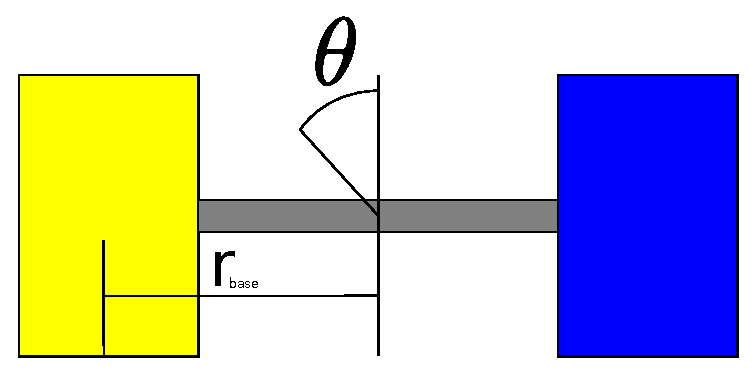
\includegraphics[width=0.7\columnwidth]{chapters/img/base_math_model.eps}
    \caption{Modelling of the base as two wheels connected with a rod, where $\theta$ is the angle to the line}
    \label{fig:base_math_model}
\end{figure}
%base_math_model.eps

Given the use of small-angles approximation\footnote{Which will be assumed since the robot will be operating on a grid with hard coded functions for turning at QR-codes}, the angular velocity can be written as:

\begin{equation}
    \theta = \frac{V_L-V_R}{2r_{b}}t
\end{equation}


\noindent Using equations \eqref{eq:base_system_eq1}-\eqref{eq:base_system_eq2} a system can be built for simulations in matlab, using rate of change and max/min value limiters for simulations of the motors physical restrictions.

%%%%%%%%%%%%%%%%%%%%%%%%%%%%%%%%%


\section*{Camera vision and calibration}
In this section it is outlined the theory behind the camera vision system. 
How points in a 3D-space are projected on a 2D-plane, calibration and distortion correction. 
\subsection*{Camera model}
\subsection*{Distortion}



%\section{Modeling}	
%

%%%%%%%%%%%%%%%% arm kinematics %%%%%%%%%%%%%%

\begin{figure}[H]
    \centering
    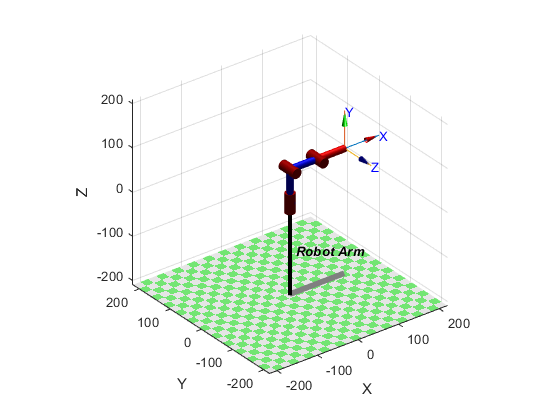
\includegraphics[width=0.7\columnwidth]{chapters/img/robot_arm.png}
    \caption{Placeholder image for the robotic arm?.}
    \label{fig:robotic_manipulator_general}
\end{figure}


\section*{Manipulator Kinematics} %Niklas
Kinematics is what describes the motion of rigid bodies and points in space. 

\subsection*{Backgroud}
\subsection*{Rigid body transformation}
In general any position can be described by translation along three axes and rotation along these same axes. These translations/rotations can be described by a matrix
\begin{equation}
    T = 
    \begin{bmatrix}
        R & d \\
        \bf{0} & 1
    \end{bmatrix}
\end{equation}
where \(R\) is a 3 x 3 rotation matrix and \(d\) a 3 x 1 translation matrix. This implies that any transformation could be characterized by six parameters, three for the translation and three for the rotation. \cite{spong}


\subsection*{Denavit-Hartenberg Convention}
A common approach for selecting the coordinate frames of reference for each joint in a robotic arm is the Denavit-Hartenberg convention. This allows the transformation matrix for each joint to be expressed as
\begin{equation}
    A_i = Rot_{z}(\theta_i) \cdot Trans_{z}(d_i) \cdot Trans_{x}(a_i) \cdot Rot_{z}(\alpha_i)
    \label{eqn:DH-transformation}
\end{equation}
that consists of the four basic transformations
\begin{equation}
    Rot_z(\theta_i) = 
    \begin{bmatrix}
        cos(\theta_i) & -sin(\theta_i) & 0 & 0 \\
        sin(\theta_i) & cos(\theta_i) & 0 & 0 \\
        0 & 0 & 1 & 0 \\
        0 & 0 & 0 & 1
    \end{bmatrix}
\end{equation}
\begin{equation}
    Trans_z(d_i) = 
    \begin{bmatrix}
        1 & 0 & 0 & 0 \\
        0 & 1 & 0 & 0 \\
        0 & 0 & 1 & d_i \\
        0 & 0 & 0 & 1
    \end{bmatrix}
\end{equation}
\begin{equation}
    Trans_x(\alpha_i) = 
    \begin{bmatrix}
        1 & 0 & 0 & \alpha_i \\
        0 & 1 & 0 & 0 \\
        0 & 0 & 1 & 0 \\
        0 & 0 & 0 & 1
    \end{bmatrix}
\end{equation}
\begin{equation}
    Rot_z(\theta_i) = 
    \begin{bmatrix}
        1 & 0 & 0 & 0 \\
        0 & cos(\alpha_i) & -sin(\alpha_i) & 0 \\
        0 & sin(\alpha_i) & cos(\alpha_i) & 0 \\
        0 & 0 & 0 & 1
    \end{bmatrix}.
\end{equation}


Where the parameters \(\theta_i\), \(a_i\), \(d_i\) and \(\alpha_i\), known as DH-parameters, characterize each joint. To allow the transformation for each joint to be represented by only four parameters, compared to the six parameters that is required in general, there are some restrictions on how the coordinate frames can be chosen. To comply with the DH-convention, the following must be satisfied.
\begin{itemize}
    \item The axis \(x_{1}\) is perpendicular to the axis \(z_0\)
    \item The axis \(x_{1}\) intersects the axis \(z_0\)
\end{itemize}
where it is assumed that two frames are given, frame 0 and frame 1, and the transformation from equation \ref{eqn:DH-transformation} transforms a coordinate from frame 1 into a coordinate in frame 0.\cite{spong}



\subsection*{Kinematic Chain} %A1*A2*...
A robotic manipulator can be described by a set of joints with links between them where a homogeneous transformation matrix \(A_i\) that describes the transformation with respect to the previous joint exists for each joint. This means that a transformation that describes the position and orientation of joint \(j\) with respect to a joint \(i\) to a can be found by a transformation matrix \cite{spong}
\begin{equation}
    \begin{cases}
        T_j^i = A_{i+1}A_{i+2}...A_{j-1}A_{j}, \text{  if \(i < j\) } \\
        T_j^i = I, \text{  if \(i = j\) } \\
        T_j^i = (T_i^j)^{-1}, \text{  if \(i > j\) }
    \end{cases}
    \label{eqn:Kinematic_chain_spong}
\end{equation}



\subsection*{Forward Kinematics}
Forward kinematics is the problem of finding the position and orientation of the end effector.

Since a manipulator can be seen as a kinematic chain the problem of finding the position and orientation of the end effector can be solved by finding the transformation matrices in equation \ref{eqn:Kinematic_chain_spong}.



\subsection*{Inverse Kinematics}
The problem of finding the joint states required for achieving a desired pose is called inverse kinematics. For some simple kinematic chains an analytical solution exists, but in general a numerical approach might be required. 

%we have for joints, three needed for position. geometric approach for finding the position. then joint for is used to control the pitch of the EOF





\subsection*{Workspace}
A robotic manipulator will not be able to reach all points in space since it has a fixed size. It will not even be able to reach all mathematically reachable points since each joint (usually) have some restrictions on how it can rotate/translate. The physically reachable space is defined as the workspace of the manipulator. %source might be needed here
\\




%%%%%%%%%%%%%%%%%%%%%%%%%%%%%%%%%%%%%%%%%%%%%%%%%%%%%%%%%%%%%%%%
%%%%%%%%%%%%%% Kinematics Implementation %%%%%%%%%%%%%%%%%%%%%%%
%%%%%%%%%%%%%%%%%%%%%%%%%%%%%%%%%%%%%%%%%%%%%%%%%%%%%%%%%%%%%%%%
\subsection*{Implementation}

\subsection*{Denavit-Hartenberg Convention}
In table \ref{tab:DH-table} the DH-parameters that was used for the robotic manipulator, seen in figure \ref{fig:robotic_manipulator_general}, are listed.
\begin{table}[H]
    \centering
    \caption{The Denavit-Hartenberg parameters used for the robotic manipulator.}
    \begin{tabular}{c | c c c c c}
        \(i\) & \(\theta_i\) [rad] & \(d_i\) [mm] & \(a_i\) [mm] & \(\alpha_i\) [rad] \\
        \hline
        \(1\) & \(\theta_1\) & \(75\) & \(0\) & \(\pi / 2\) \\
        \(2\) & \(\theta_2\) & \(0\) & \(67.5\) & \(0\) \\
        \(3\) & \(\theta_3\) & \(0\) & \(67.5\) & \(0\) \\
        \(4\) & \(\theta_4\) & \(0\) & \(65\) & \(0\) \\
    \end{tabular}
    \label{tab:DH-table}
\end{table}



\subsection*{Forward Kinematics}
The transformation matrices from equation \ref{eqn:DH-transformation} for each joint can be multiplied together
\begin{equation}
    T_{end} = A_1 \cdot A_2 \cdot A_3 \cdot A_4
\end{equation}
where \(A_1\) - \(A_4\) are calculated from equation \ref{eqn:DH-transformation} to find the pose \(T_{end}\) of the end effector and thereby solving the forward kinematic problem.


\subsection*{Inverse Kinematics}
To solve the inverse kinematics for the position of a three joint manipulator a geometric method can be used to find an analytical solution. The required angles to achieve a desired position \((x_d, y_d, z_d)\) in an elbow-up configuration are \cite{Lec14_mit_Manipulation}

\begin{equation}
    \begin{cases}
        \theta_1 = Atan(x, y) \\
        \theta_3 = Atan(D, +\sqrt{1 - D^2}) \\
        \theta_2 = Atan(\sqrt{x_d^2 + y_d^2}, z_d - d_1) \\- Atan(a_2 + a_3 \cdot D, a_3 \cdot \sqrt{1 - D^2}) %fix
    \end{cases}
\end{equation}
where \(Atan(x, y)\) is the two argument arctangent function \cite{inverse_tangent_wolfram} and 

\begin{equation}
    D = \frac{x_d^2 + y_d^2 + (z_d - d_1)^2 - a_2^2 - a_3^2}{2 a_2 a_3}
\end{equation}
and \(a_2\), \(a_3\), and \(d_1\)   are the corresponding DH-parameters.



\subsection*{Workspace}
The robotic manipulator seen in figure \ref{fig:robotic_manipulator_general} has the following limitations for the first three joints
\begin{equation}
    \begin{cases}
        -100^\circ < \theta_1 < 100^\circ \\
        -100^\circ < \theta_2 < 100^\circ \\
        -100^\circ < \theta_3 < 100^\circ 
    \end{cases}
    \label{eqn:workspace_limits_angles}
\end{equation}
and a simulated 2D slice of the workspace can be seen in figure \ref{fig:workspace_simulated}. The full workspace can be formed by rotating this 2D slice around the z-axis according to the limitations on \(\theta_1\) from equation \ref{eqn:workspace_limits_angles}.


\begin{figure}[H]
    \centering
    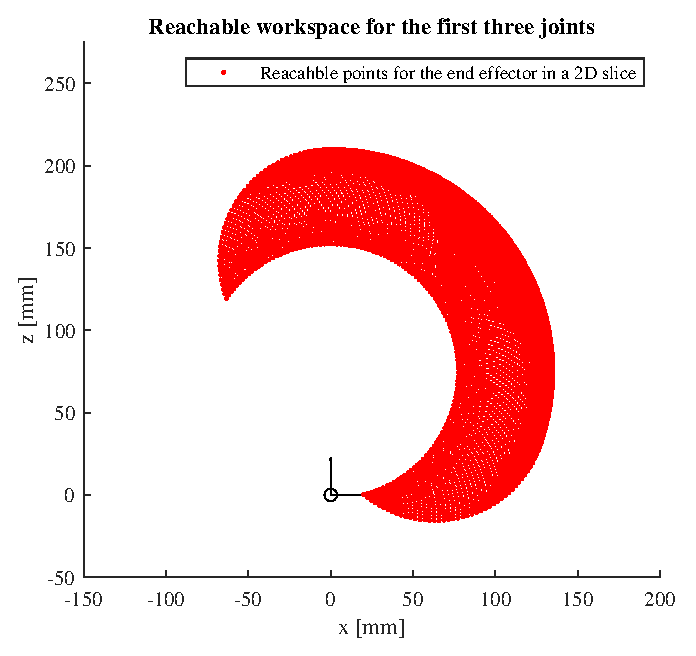
\includegraphics[width=0.7\columnwidth]{chapters/img/workspace.eps}
    \caption{A simulated 2D slice of the workspace for the three jointed manipulator.}
    \label{fig:workspace_simulated}
\end{figure}
%chapters/img/workspace.eps




%%%%%%%%%%%%%%%% arm kinematics end %%%%%%%%%%%%%%













\section*{Base}

The motors will be connected to tracks on the robot and can therefore be modelled as two wheels connected with a rod, as seen in figure \ref{fig:base_math_model}.\\ 
Deriving a mathematical model is straight forward if we can read the encoders from the motors. From the encoders we would be able to get both the length the robot has traveled and more importantly the individual speed each motor rotates with. The speed for the individual motor is given by: 

\begin{equation}
    v_m=\frac{2\pi r_{wh}/N_{enc}}{\Delta t}
    \label{eq:base_system_eq1}
\end{equation}

\noindent Where $N_{enc}$ is the number of encoders on the motor, $r_{wh}$ is the radius of the driving wheel and thickness of the track and $\Delta t$ is the time between the previous encoder reading and the most recent one. By doing this for both the left and right motor we can find how fast the robot is moving along the line by:

\begin{equation}
    \overline{v}= \frac{v_L+v_R}{2}(-\cos \theta \hat{i}+ \sin \theta \Hat{j})
\end{equation}

\noindent Where the $y$-axis parallel to the line. In a similar fashion the angular velocity can be calculated using:

\begin{equation}
    \Dot{\theta} = \frac{v_R-v_L}{2r_{b}}
    \label{eq:base_system_eq2}
\end{equation}

\noindent Where $r_{b}$ is the distance from the center of the base to the wheels. From this and figure \ref{fig:base_math_model} it's easy to see that the change of angle then becomes:

\begin{equation}
    \theta = sin^{-1}\left(\frac{V_L-V_R}{2r_{b}}t\right)
\end{equation}

\begin{figure}[H]
    \centering
    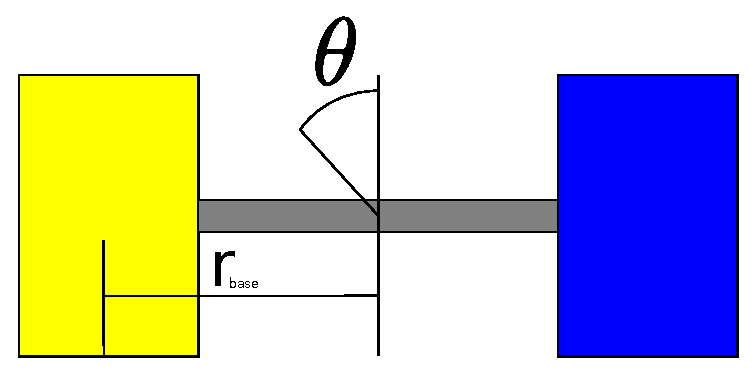
\includegraphics[width=0.7\columnwidth]{chapters/img/base_math_model.eps}
    \caption{Modelling of the base as two wheels connected with a rod, where $\theta$ is the angle to the line}
    \label{fig:base_math_model}
\end{figure}
%base_math_model.eps

Given the use of small-angles approximation\footnote{Which will be assumed since the robot will be operating on a grid with hard coded functions for turning at QR-codes}, the angular velocity can be written as:

\begin{equation}
    \theta = \frac{V_L-V_R}{2r_{b}}t
\end{equation}


\noindent Using equations \eqref{eq:base_system_eq1}-\eqref{eq:base_system_eq2} a system can be built for simulations in matlab, using rate of change and max/min value limiters for simulations of the motors physical restrictions.

%%%%%%%%%%%%%%%%%%%%%%%%%%%%%%%%%


\section*{Camera vision and calibration}
In this section it is outlined the theory behind the camera vision system. 
How points in a 3D-space are projected on a 2D-plane, calibration and distortion correction. 
\subsection*{Camera model}
\subsection*{Distortion}
	

\section{Machine Vision}	
In order for the robot to navigate the factory floor in a reliable and cost-effective manner a system using lines and QR codes is proposed.
Ideally, the robot should be able to travel between points in an arbitrary grid.
A grid is made up of multiple connected colored lines.
At every point where lines intersect a QR code containing a coordinate is placed.

To facilitate this, a machine vision system using a RGB camera is proposed. The machine vision system consists of two major components.
One component is a line following algorithm which can take an image of a colored line and produce an angle between this line and the base of the robot. This angle is then used in the motor controller.
The second component is a QR code reader, this makes it possible for the robot to behave in different ways depending on the contents of the approached QR code.
These components are used in conjunction to allow the robot to travel between the points in the grid.

\section*{Line Following}
The camera is placed in a top down configuration. This makes it possible for the camera output to be regarded as a 2D surface.
The process of producing an angle from an input image of a colored line is divided into four different steps which can be summarized as follows:

\begin{enumerate}
	\item Crop out a horizontal slice
	\item Create color mask to extract line
	\item Determine center point of line using image moment
	\item Calculate angle between center point and robot base.
\end{enumerate}

% Step 1
To begin with a horizontal slice of the captured image is cropped out at a fixed vertical offset, $y_0$. This slice is visualized by the two horizontal red lines in figure \ref{fig:mv_frame}.
All remaining processing is done on this slice.
\\ \\
% Step 2
The image is then converted to HSV color space and a predetermined color mask is applied to extract only the pixels with the same color as the followed line.
This step produces a new binary image where each pixel is represented with either a 1 or a 0 depending on if the original pixel was inside the predetermined color range or not.
A visualization of this binary image is seen in the rightmost part of figure \ref{fig:mv_frame}.
This binary image is then used as the input for the next step.
\\ \\
% Step 3
To find the centroid of this binary image the \emph{moment} is calculated. The image moment is in some sense analogous to the concept of \emph{center of mass} used in physics. It is defined as
\begin{equation}
	m_{p q}=\int_{-\infty}^{\infty} \int_{-\infty}^{\infty} x^{p} y^{q} I(x, y) \mathrm{d} x \mathrm{~d} y
\end{equation}
where $I(x,y)$ denotes the intensities of the image \cite{moment}.
This formula is discretized in order to be usable with an array of pixels
\begin{equation}
	M_{p q}=\sum_{x} \sum_{y} x^{p} y^{q} I(x, y).
\end{equation}
The center of the image in the horizontal direction is then given by
\begin{equation}
	\bar{x} = \frac{m_{10}}{m_{00}}.
\end{equation}
\\ \\
% Step 4
All that remains to do is then to calculate the angle between the horizontal axis and the line drawn between the point $(\bar{x}, y_0)$ and the base of the robot, denoted as $(x_r, y_r)$.
The angle $\alpha$ is then given by
\begin{equation}
	\alpha = \tan^{-1}\left(\frac{y_0 - y_r}{\bar{x} - x_r}\right).
\end{equation}
The angle output is visualized in figure \ref{fig:mv_frame}.
This process is repeated for every captured frame and will produce a continuous stream of angles which can then be used by other components of the robot.

\section*{QR Code Reader}
In order to provide the robot with additional positional information QR codes are used.
The basic QR code functionality is provided with the use of the \emph{ZBar}\cite{zbar} library.
Functionality to extract information about from which cardinal direction a QR code is being read is implemented manually.

% Does this go under MV or some other base movement section?
Each QR contains information of the form $\{x,y\}$, where $x$ and $y$ are the Cartesian coordinates of the QR code in the grid.
An internal representation of the entire grid is stored in the form of an adjacency matrix.

By taking the relative position of two adjacent QR codes together with the direction from which the robot is approaching the current QR code it is possible to calculate which way the robot must turn to reach the next QR code.

As with the line following algorithm each frame is processed and scanned for QR codes.
The contents of the QR code, the position of the QR code and the cardinal direction from which the QR code is approached is sent to be used by the other components of the robot.	

\section{Motion}	
\section*{Robot Arm Path Planning} 
If a robot manipulator is required to visit specific discrete points, waypoints, path planning is the problem of deciding how to move between these points. Planning the path is also important to ensure the movements are smooth, meaning that, since we "control" the speed of each joint, the desired positions and velocities should be continuous.%Path planning is very important, a smooth path will make a manipulator move better :) %is right
\subsection*{Interpolation}
One method of interpolating between points is to use cubic spline interpolation. A spline \cite{spline_wolfram} is a piecewise polynomial function and consequently a cubic spline is a function consisting of piecewise cubic polynomials. A cubic polynomial will ensure a smooth movement since its first derivative, the velocity, will be continuous. To ensure that each required point is visited the bounding values for each cubic function are set to zero \cite{cubic_spline_wolfram}.
\subsection*{Joint Space interpolation or Cartesian Motion}
The interpolation can take place in joint space or in cartesian space. Joint space interpolation means that the waypoints are expressed as joint values, angle of rotation if the joint is a revolute joint and distance if the joint is a prismatic joint.
The interpolation is then calculated between these joint values. Cartesian motion means that the waypoint are expressed as cartesian coordinates and that the interpolation takes place in cartesian space.
%Joint space - interpolate the joint values
%Cartesian motion - interpolate in 3D space -> convert to joint angles
\subsection*{Implementation} %Pre recorded path
The robotic manipulator, shown in figure \ref{fig:robotic_manipulator_general}, has a number of waypoints that it is required to visit. The desired waypoints are expressed in joint values, and a cubic spline interpolation is used to interpolate between these joint space waypoints. The path for picking up and placing the object can be seen in figure \ref{fig:pickup_path_interpolated} and \ref{fig:place_path_interpolated} respectively.

\begin{figure}[H]
    \centering
    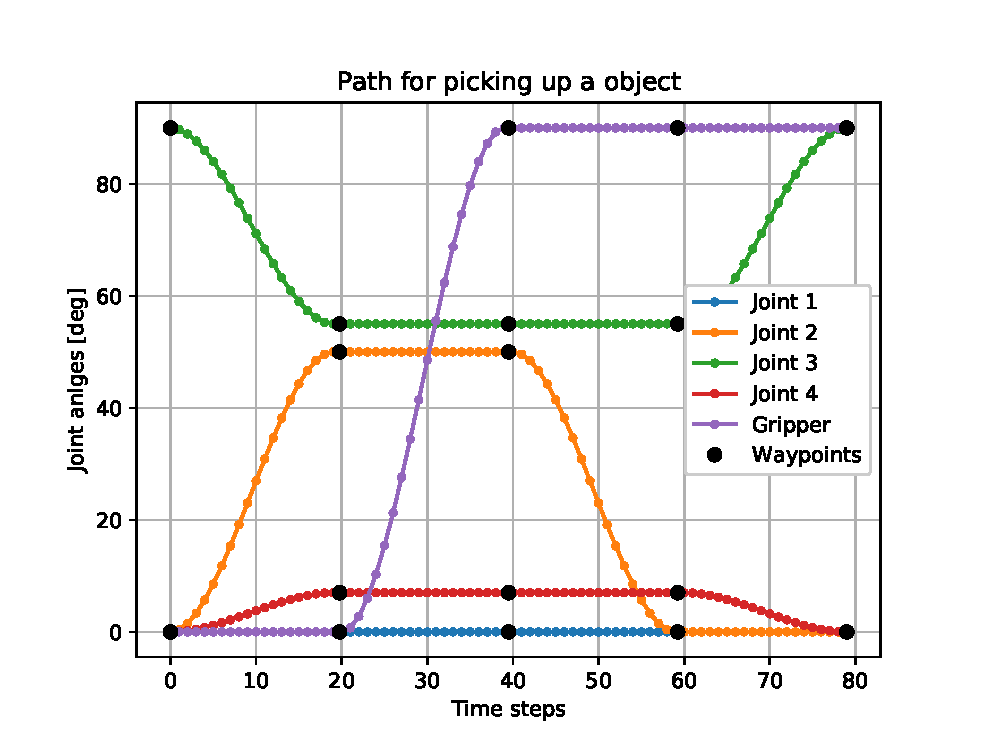
\includegraphics[width=0.5\textwidth]{chapters/img/pickup_path.eps}
    \caption{Path showing the joint values required for picking up the object.}
    \label{fig:pickup_path_interpolated}
\end{figure}


\begin{figure}[H]
    \centering
    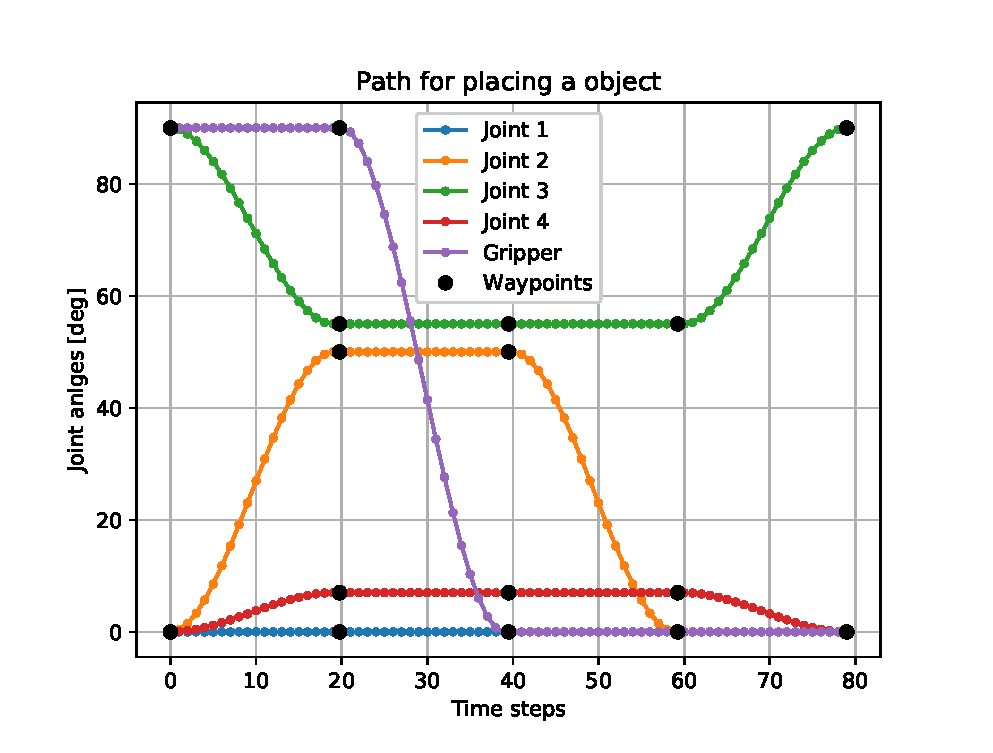
\includegraphics[width=0.5\textwidth]{chapters/img/place_path.eps}
    \caption{Path showing the joint values required for placing the object.}
    \label{fig:place_path_interpolated}
\end{figure}






\section*{Base}


	

\section{Experiment}	
\section*{Prototype components}
\section*{Movable base evauation}
\section*{Arm evaluation}
\section*{Gripping evaluation}
\section*{Sensor evaluation}	

\section{Evaluation}
\subsection{Engineering challenge}
Performance of the robot during navigation on the setup shown in Fig. \ref{fig:factory_setup} was evaluated with the following criterias

\begin{itemize}
    \item Autonomy of the robot
    \item Speed and navigation
    \item Pickup / drop-off performance
\end{itemize}

The test were performedd at Luleå University of Technology at EISLAB with a local Arrowhead cloud and private network. The robot was able to navigate the factory floor and perform the action but moved slowly. This is because the Dynamixel motors used to translate the robot are slow. Communicating with Arrowhead was working and the test was proved successfull. A video with the whole run can be seen here: https://www.youtube.com/watch?v=YoAFspEC2no. 
We can't do the evaluation without mentioning som limitations. The speed of the robot is mentioned above but also because of the line following algorithm the robot can get lost if it ever loses the line. This could be prevented with an external navigation system such as GPS, Ultra Wide Band (UWB) or simliar. 

\subsection{Factory setup}
In this project we also propose how a factory test-bed can be designed. In this solution the main components are the colored lines and QR-codes. The ain advantage of this setup is that it's very flexible. First of all the path can have any shape and the QR-codes can contain any information. Further, more colors can be utilized to identify different parts of the factory, stop certain robots from following them or use lines with multiple colors to determine the orientation of the robot while following the path. While flexible thhis solution may get complicated and hard to alter for very big factories. Also a fast and easy system to register QR-codes and information would need to be implemented. 

\section{Conclusions}	
Conclusions of the robot and the course (?)
Is our design good?
Is Arrowhead good? 
	





\section*{Conceptual design}	

\newpage	
\appendix	
% !TeX root = ../main.tex

\section*{Martin Blaszczyk}
Martin is a 5th year Y-student with interest in Control och Mechatronics. 
In this course he'll take the role of the Project Leader where the main objectives
are to keep focus on the goal, hold meetings and an overall oversight of the project. 
As for the technical part the main interest will be in machine vision together with
Edward K. to use cameras or other sensors to localize external objects for the 
robot to grip, avoid or approach.

\section*{Edward Cedgård}

Master in  electronic systems and control engineering.
Edward's main task is to design the robotic arm and gripper mechanism together with Niklas. 
Tasks as deriving the kinematic equations, and implementation using forward and inverse kinematics.
Choise of motors, armdesign, communication with motors using serial communication. 

\section*{Niklas Dahlquist}
Niklas is studying his fifth year at the Engineering physics and electrical engineering student program.

His main focus will be to work with Edward Cedgård to evaluate the gripping mechanism and if necessary design new components and model the corresponding control system to be able to lift up and hold the target object.

\section*{Edward Källstedt}
Currently studying his fourth year in the Master Programme in Computer Science and Engineering.
A fan of making things secure, fast, scalable, and well-documented. Primarily interested in
low level software development. Will initially work on the machine vision implementation 
together with Martin. In addition to machine vision specifically this work will also consist
of robot localization and collision avoidance. As the project progresses he will take on more
general software problems that might arise. The first week will be spent researching different
computer vision technologies.


\section*{Albin Martinsson}


\section*{Måns Norell}


\chapter{Working together}
\section*{Project structure}
To keep the project going and have an organized structure the project is divided 
in different parts, or subprojects. Each group member is either alone or in group responsible for each part of the project which coincides with their interests. 
\begin{itemize}
    \item Arrowhead
    \item Machine vision and localization of external objects
    \item Gripping tool
    \item Movable base
\end{itemize}

\section*{Meetings}
Every week the group will be meeting on Mondays and Tuesdays to catch up and support each other. This scheme may change in the future if needed. 
The Monday meetings will have the following agenda where the goal is to catch up with the whole project group and discuss the project
\begin{itemize}
    \item Status of work done the previous week by each member
    \item Preparation for the seminar
    \begin{itemize}
        \item Discussion of the previous seminar meeting
        \item How the weeks work has been coinciding with the seminar feedback
        \item Questions to ask the teachers
        \item Questions to ask the other group
        \item Who does what during the Tuesday seminar
    \end{itemize}
    \item Other
\end{itemize}
The Tuesday meeting will be after the seminar to collect and reflect over the 
feedback from the teachers and the other group. Also a status on the work planned to be done 
the coming week will be discussed so that each member has an overview of what 
the other members are doing. The meetings will have the following agenda
\begin{itemize}
    \item What feedback did the teachers give
    \item What feedback did he other group give 
    \item Feedback to each other withing the group
    \item Work to be done the following week
    \item Other 
\end{itemize}
As mentioned, this meeting structure may be subject to changes if needed and of course if any member of the group wants to work from home a video call will be organized. 











	


\bibliographystyle{IEEEtran}	
\bibliography{bibliography.bib}	


\end{document}	

